\documentclass[letterpaper,10pt]{article}

\usepackage[utf8]{inputenc}
\usepackage[spanish]{babel}
\usepackage{fontenc}
\usepackage[dvipdfmx]{graphicx}
\usepackage{bmpsize,wrapfig,xcolor}
\usepackage{fullpage}
\usepackage{amssymb}
\usepackage[hidelinks]{hyperref}

% Para evitar que se indente solo a cada rato
\setlength\parindent{0pt}

\begin{document}
	\begin{titlepage}

		\begin{wrapfigure}{R}{0.3\textwidth}
			
\includegraphics[width=0.3\textwidth]{logoFCFM.png}
		\end{wrapfigure}

		\noindent \phantom - % "Hax" para que quede alineada la imagen con el texto

		Universidad de Chile

		Facultad de Ciencias Físicas y Matemáticas

		Depto. de Ciencias de la Computación

		CC4102 - Diseño y Análisis de Algoritmos

		\vfill

		\begin{center}
			\begin{Huge}
				{\textbf{Tarea 2}}
			\end{Huge}
		\end{center}

		\vfill

		\begin{flushright}
			\begin{tabular}{lll}
				Integrantes	&:	& Rodrigo Delgado\\
						&	& Belisario Panay\\
						&	& Gabriel Sanhueza\\
				Profesor	&:	& Gonzalo Navarro\\
				Ayudantes	&:	& Sebastián Ferrada\\
						&	& Willy Maikowski\\
				Auxiliar	&:	& Jorge Bahamondes\\
			\end{tabular}
		\end{flushright}

	\end{titlepage}

	% % % % % % % % % % % % % % % % % % % % % % % % % % % % % % % % % % % % % % % % % % % % % % % % % % % % % % % % % % % % % % % % % % % % % % % % % % % % % % % % % % % % % % % % % %
	\newpage
	% % % % % % % % % % % % % % % % % % % % % % % % % % % % % % % % % % % % % % % % % % % % % % % % % % % % % % % % % % % % % % % % % % % % % % % % % % % % % % % % % % % % % % % % % %

	\tableofcontents

	% % % % % % % % % % % % % % % % % % % % % % % % % % % % % % % % % % % % % % % % % % % % % % % % % % % % % % % % % % % % % % % % % % % % % % % % % % % % % % % % % % % % % % % % % %
	\newpage
	% % % % % % % % % % % % % % % % % % % % % % % % % % % % % % % % % % % % % % % % % % % % % % % % % % % % % % % % % % % % % % % % % % % % % % % % % % % % % % % % % % % % % % % % % %

	\section{Introducción}

	Un \textit{suffix tree} es un \textit{trie} (Trie: Estructura ordenada en forma de árbol) comprimido, el cual contiene todos los sufijos de un texto dado como sus llaves, y sus posiciones en el
	texto como sus valores.

	En el presente informe se muestra el diseño, implementación y experimentación del algoritmo de Ukkonen, el cual es un algoritmo de orden lineal para la creación de Suffix Trees,
	formada por Nodos que poseen información interna y referencias a sus hijos.

	En particular el algoritmo de Ukkonen para un Suffix Tree almacena los sufijos de un string en forma de árbol, de modo que cada arco contiene los caracteres para formar una palabra, y
	agregando caracteres sucesivos hasta que el árbol está completo.
	Por tanto, al momento de buscar, si se llega a una hoja (nodo terminal) es porque se recorrieron los arcos necesarios para formar un sufijo.

	La idea de la tarea es que el algoritmo a desarrollar es \textit{on-line}, de orden lineal ($O(n)$) y con una implementación más sencilla con respecto a algoritmos similares (algoritmo de Weiner
	y algoritmo de McCreight).

	\subsection{Problema a resolver}

	Un algoritmo estándar de creación de Suffix Tree toma tiempo $O(n^3)$, mientras que el algoritmo de Ukkonen toma tiempo $O(n)$.
	El problema consiste en realizar los pasos necesarios para la buena implementación del algoritmo, ya que pequeños errores en código pueden producir un algoritmo de mayor orden de magnitud
	y con ello se falla en el objetivo.

	Los pasos para realizarlos estan detallados en el enunciado de la tarea y en el \textit{paper} de Esko Ukkonen, creador del algoritmo.

	\subsection{Hipótesis}

	Si bien es un algoritmo lineal, el algoritmo posee una constante que hace que el tiempo pueda crecer de manera rapida. Además, como el algoritmo será escrito en Java como lenguaje,
	la eficiencia del algoritmo se podría ver reducida, dado que el \textit{garbage collector} usa la CPU para realizar sus funciones. Se espera demostrar que la constante del algoritmo
	varía con respecto al largo por motivos externos al algoritmo, lo cual se puede demostrar si para números pequeños el algoritmo sí demuestra un comportamiento lineal.

	% % % % % % % % % % % % % % % % % % % % % % % % % % % % % % % % % % % % % % % % % % % % % % % % % % % % % % % % % % % % % % % % % % % % % % % % % % % % % % % % % % % % % % % % % %
	\newpage
	% % % % % % % % % % % % % % % % % % % % % % % % % % % % % % % % % % % % % % % % % % % % % % % % % % % % % % % % % % % % % % % % % % % % % % % % % % % % % % % % % % % % % % % % % %

	\section{Diseño Teórico}

	Se crearon distintas clases de Java para cada comportamiento dentro del Suffix Tree, y una clase principal Main, donde se hacen las pruebas.

	\subsection{Main}

	En Main se crea un archivo de \textit{logging} para registrar el tiempo de creación del Suffix Tree y los resultados de búsqueda, a partir de un texto leído desde el disco.
	En particular:
	\begin{itemize}
		\item El texto leído se preprocesa (se eliminan puntuaciones, espacios, saltos de línea y todo lo que no corresponda al \textit{regex} [a-ZA-Z]).
		\item Se crea el Suffix Tree usando el algoritmo de Ukkonen.
		\item Se registra el tiempo de creación.
		\item Se generan palabras aleatorias del texto, para buscarlas usando el Suffix Tree.
		\item Se registran los resultados de búsqueda.
	\end{itemize}


	\subsection{Ukkonen}

	// TODO: Explicar cómo lo hicimos para hacer que el algoritmo funcionara

	\subsection{Otras clases}

	// TODO: Limpiar código de las clases que no se usan, para poner aquí las que sí usamos

	% % % % % % % % % % % % % % % % % % % % % % % % % % % % % % % % % % % % % % % % % % % % % % % % % % % % % % % % % % % % % % % % % % % % % % % % % % % % % % % % % % % % % % % % % %
	\newpage
	% % % % % % % % % % % % % % % % % % % % % % % % % % % % % % % % % % % % % % % % % % % % % % % % % % % % % % % % % % % % % % % % % % % % % % % % % % % % % % % % % % % % % % % % % %

	\section{Presentación de los Resultados}

	\subsection{Tiempo de Creación del Suffix Tree}

	// TODO: Mostrar cuanto se tarda en crear un suffix tree, para N = 2 ** 15..21 palabras (aprox).

	\begin{center}
		\begin{tabular}{|c|c|c|}
			\hline
			Largo del texto & Tiempo de Construcción & Operaciones por fase\\
			\hline
			$2^{15}$ & X & X\\
			\hline
			$2^{16}$ & X & X\\
			\hline
			$2^{17}$ & X & X\\
			\hline
			$2^{18}$ & X & X\\
			\hline
			$2^{19}$ & X & X\\
			\hline
			$2^{20}$ & X & X\\
			\hline
			$2^{21}$ & X & X\\
			\hline
		\end{tabular}
	\end{center}

	\begin{center}
		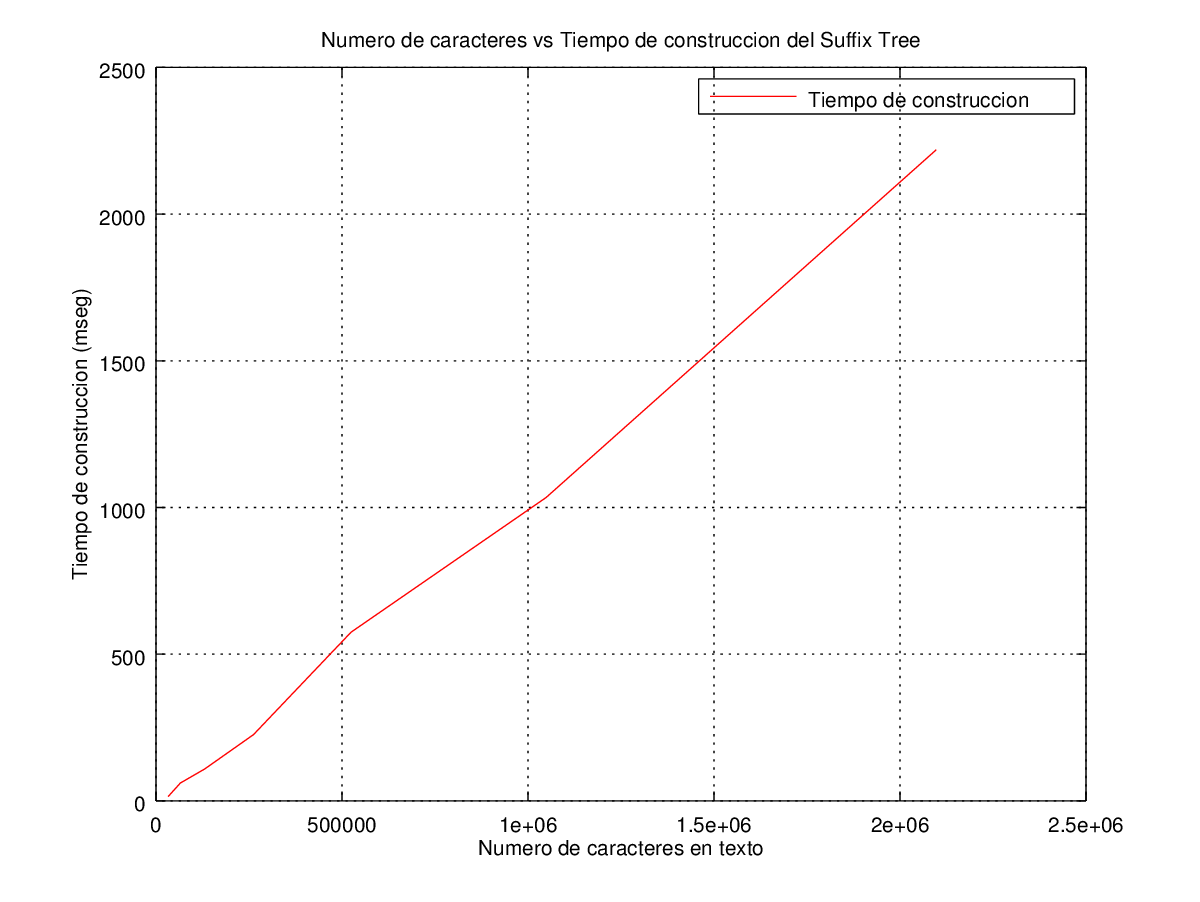
\includegraphics[width=0.8\textwidth]{fig1.png}

		Figura 1:
	\end{center}

	% % % % % % % % % % % % % % % % % % % % % % % % % % % % % % % % % % % % % % % % % % % % % % % % % % % % % % % % % % % % % % % % % % % % % % % % % % % % % % % % % % % % % % % % % %
	\newpage
	% % % % % % % % % % % % % % % % % % % % % % % % % % % % % % % % % % % % % % % % % % % % % % % % % % % % % % % % % % % % % % % % % % % % % % % % % % % % % % % % % % % % % % % % % %

	\subsection{Desempeño de operación \textit{Buscar}}

	// TODO: Mostrar cuanto se demora en buscar N = (2 ** 15..21) / 10 palabras (aprox).

	\begin{center}
		\begin{tabular}{|c|c|c|}
			\hline
			Número de palabras & Largo promedio del patrón & Tiempo de búsqueda\\
			\hline
			$2^{15}$ & X & X\\
			\hline
			$2^{16}$ & X & X\\
			\hline
			$2^{17}$ & X & X\\
			\hline
			$2^{18}$ & X & X\\
			\hline
			$2^{19}$ & X & X\\
			\hline
			$2^{20}$ & X & X\\
			\hline
			$2^{21}$ & X & X\\
			\hline
		\end{tabular}
	\end{center}

	\begin{center}
		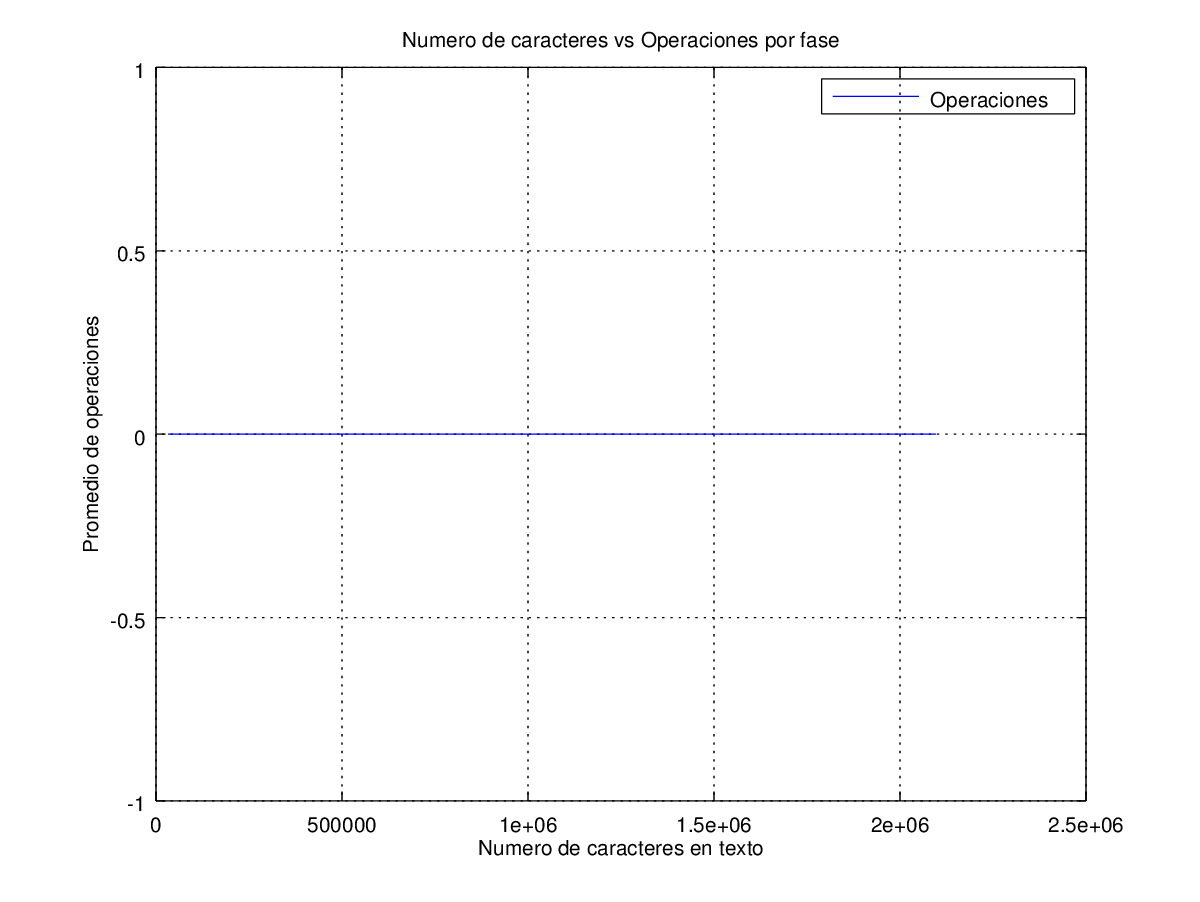
\includegraphics[width=0.8\textwidth]{fig2.png}

		Figura 2:
	\end{center}

	\begin{center}
		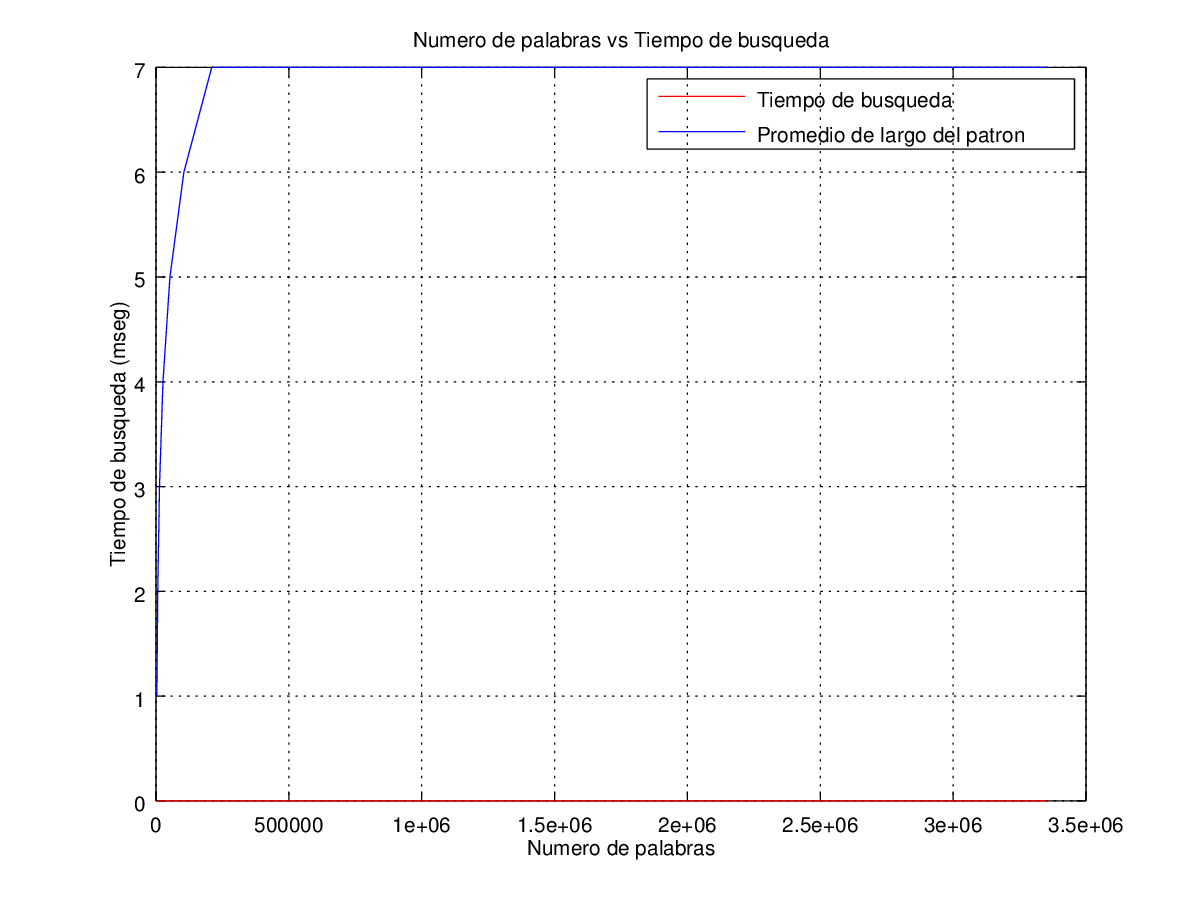
\includegraphics[width=0.8\textwidth]{fig3.png}

		Figura 3:
	\end{center}

	% % % % % % % % % % % % % % % % % % % % % % % % % % % % % % % % % % % % % % % % % % % % % % % % % % % % % % % % % % % % % % % % % % % % % % % % % % % % % % % % % % % % % % % % % %
	\newpage
	% % % % % % % % % % % % % % % % % % % % % % % % % % % % % % % % % % % % % % % % % % % % % % % % % % % % % % % % % % % % % % % % % % % % % % % % % % % % % % % % % % % % % % % % % %

	\section{Análisis y Conclusiones}

	\subsection{Construcción del Suffix Tree}

	// TODO: Verificar si el Suffix tree fue lineal o no

	\subsection{Búsqueda en el Suffix Tree}

	// TODO: Verificar si los tiempos están acotados o se fueron a la chu*** cada vez que aumentamos el número

	\subsection{Conclusiones}

	// TODO: Resumir lo ``aprendido'' (?)

\end{document}
